\documentclass[prl,aps,twocolumn,showpacs,twocolumngrid,superbib]{revtex4}

\usepackage{graphicx}
\usepackage{amsfonts}
\usepackage{amsmath}
\usepackage{bm}
\usepackage{alltt}
\usepackage{fancyhdr}

\pagestyle{fancy}

\newcommand{\commentoutA}[1]{}
\newcommand{\commentoutB}[1]{#1}

\begin{document}

\title{\emph{Ab-inito} Linear Scaling Response: \\ Computation of the Electric Polarizability}

\author{Val\'ery Weber}
\altaffiliation[Also at ]{Dept. of Chemistry, University of Fribourg, 1700 Fribourg, Switzerland}
\email{vweber@t12.lanl.gov}
\author{Anders M. N. Niklasson}
\author{Matt Challacombe}
\affiliation{Los Alamos National Laboratory, Theoretical Division, Los Alamos 87545, New Mexico, USA.}

\date{\today}

\begin{abstract}
A linear scaling method for calculation of static {\em ab inito} response theory
 within self-consistent field theory 
is developed and applied to calculation of the static electric polarizability. 
 The method is based on the density matrix 
perturbation theory [Niklasson and Challacombe, cond-mat/0311591], which obtains
 response functions
 {\bf explicitly by recursion based on spectral projection.}
% directly via an iterative approach to spectral projection.
 The accuracy and the efficiency of
 the linear scaling method is demonstrated 
for a series of three-dimensional water cluster at the RHF/6-31G** level of theory.
  Locality of the response 
under a global electric field perturbation is numerically demonstrated by an approximate exponential decay of
matrix elements of the density matrix derivative.
\end{abstract}

\maketitle

\footnotetext[1]{LA-UR-03-9111}

Linear scaling methods that reduce the computational complexity of 
electronic structure calculations to ${\cal O}(N)$, where $N$ is system size, 
impact disciplines that demand quantum simulation of increasingly large and complex systems
\cite{GGalli96,DBowler97,SGoedecker99,POrdejon00,VGogonea01,SWu02}. 
To date, the most successful and prolific applications of linear scaling technologies are
ground state studies involving empirical model Hamiltonians.  
{\bf To a lesser degree also ground state applications using {\em ab initio} models 
with $N$-scaling contribute to a variety of fields. These calculations
often require parallel implementations to reach levels of applicability comparable with
empirical ones.}
% To a lesser degree, ground state applications using {\em ab initio} models 
% with $N$-scaling contribute to a variety of fields, requiring in some
% cases parallel implementations to reach levels of applicability comparable with
% empirical ones. 
Beyond ground state methods, less attention has been given 
to linear scaling algorithms for the computation of dynamic and static response 
properties; the latter including the nuclear magnetic shielding tensor \cite{Pulay_1990}, 
the rotational g-tensor \cite{Helgaker_1996}, indirect spin-spin coupling constant 
\cite{Pennington_1991,Malkin_1996}, third order  properties such as the first hyperpolarizability 
\cite{Franky_1997} and polarizability derivatives such as the Raman intensity 
\cite{Lazzeri_2003,Champagne_2001}.  Dynamic  properties may be computed using 
linear scaling algorithms to propagate the density matrix \cite{SNomura97,CYam03} in 
the time domain, followed by convolution to obtain the spectral response.  In this way, 
Yam, Yokojima and Chen \cite{CYam03} have recently demonstrated linear scaling 
computation of the absorption spectra for one-dimensional polymers at the local 
density level of theory, but requiring $\sim 14,000$ time steps.  
In the static zero frequency limit, solving the coupled-perturbed self-consistent-field 
(CPSCF) equations using standard algorithms for systems larger than $\sim 100$ atoms 
is very difficult, although several algorithms have been proposed for 
solving the CPSCF equations that {\bf may}, in principle, capable of achieving a reduced scaling 
better than ${\cal O}(N^3)$\cite{COchsenfeld97,HLarsen00} {\bf REMOVE ANiklasson03}.   
In this letter, we develop the density matrix perturbation theory of  Niklasson and Challacombe 
\cite{ANiklasson03} for $N$-scaling solution of the {\em ab initio} CPSCF equations, and 
demonstrate the early onset of linear scaling for the accurate calculation of the first electric 
polarizability of three-dimensional systems using non-trivial basis sets.

Algorithms for linear scaling self-consistent-field (SCF) theory exploit the quantum locality
of non-metallic systems, manifested in the approximate exponential decay of the density matrix 
with atom-atom separation, through the effective use of sparse matrix methods and iterative 
approaches to spectral projection \cite{ANiklasson02}.   This quantum locality should, in principle,
extend also to the derivative density matrices central to the CPSCF equations.  Indeed,  
exponential decay of the derivative density matrix within SCF theory has been demonstrated numerically
for local nuclear displacement \cite{Ochsenfeld_1997}. However, standard approaches to the CPSCF equations 
\cite{Pople_1979,Sekino_1986,Dupuis_1991} do not admit exploitation of this locality, as they are based 
on perturbation of the wave function, requiring ${\cal O}(N^3)$ eigensolution and typically ${\cal O}(N^5)$ 
transformation of two-electron integrals into the eigenbasis.   Avoiding both 
eigensolution and integral transformation,  Ochsenfeld and Head-Gordon \cite{Ochsenfeld_1997} and
later Larsen et al \cite{Helgaker_2001} proposed iterative solutions to the CPSCF equations 
involving purely non-orthogonal representations.   In both of these approaches, a 
linear system of equations containing commutation relations  was obtained.  These equations
are related to the Sylvester equations, and can be re-expressed in standard form 
as the linear system $Ax=b$ using the Kronecker product formalism \cite{}.  In this form 
$A$ is a $N^2\times N^2$ matrix, $x$ is a $N^2$ vector that contains the 
density matrix derivative and $b$ a $N^2$ vector that contains the inhomogeneous
part of the response equations. However, even if the matrix $A$ is strictly diagonal, 
solution of these equations with sparse iterative methods is at best ${\cal O}(N^2)$. 

Recently, a formulation of density matrix perturbation theory has been proposed 
by Niklasson and Challacombe (NC) \cite{} that establishes a new approach to {\bf solve OR solving ?}
the CPSCF equations within the context of linear scaling spectral projection \cite{}.  
In this approach to solution of the SCF equations, a direct relationship is established between 
the density matrix $\mathcal{D}$  and the effective Hamiltonian or Fockian $\mathcal{F}$ through 
the spectral projector ({\bf Matt it is Heaviside not Heavyside ;) AMNN } step function)
 $\mathcal{D}=\theta(\tilde{\mu}I-\mathcal{F})$, 
where the chemical potential $\tilde{\mu}$ determines the occupied states via Aufbau filling.   
The density matrix and the Fockian depend on each other in a non-linear way, and are solved
iteratively, arriving at a self-consistent solution only when $[\mathcal{F},\mathcal{D}]=0$.
Spectral projection can be carried out in a number of ways \cite{}, with perhaps the best
know algorithm being McWeeny's cubic purification scheme \cite{}. 
More recently new recursive polynomial expansions of the projector have emerged, 
such as the second order trace correcting (TC2) \cite{} and fourth order trace resetting 
(TRS4) \cite{} purification.  These new methods (TC2 and TRS4) have convergence properties 
that depend only weakly on the band gap, do not require knowledge of the chemical potential
and perform well for all occupation to state ratios. In the NC approach, 
the perturbation expansion is developed within the reference groundstate projector allowing 
order by order collection of terms at each iteration, establishing a {\bf quadratically}
 convergent sequence for
the response functions.  

% We will now proceed to
{\bf In this letter we will} develop a more formal approach to linear scaling
 solution of the CPSCF equations.
For simplicity and familiarity, this approach will be outlined for the concrete case of 
perturbation by an electric field within the Hartree-Fock (HF) theory.  However, the method is 
completely general and with minor modification extensible to Density Functional (DFT), hybrid 
HF/DFT models, and to other static perturbations through high order.

Superscripts and subscripts refer to perturbation order and iteration count respectively.  
The symbols $\mathcal{D},\mathcal{F},\dots$  are  matrices in an orthogonal representation, while
$D,F,\dots$ are the corresponding matrices in a non-orthogonal basis.  We note that the transformation 
between orthogonal and non-orthogonal representations {\bf is} carried out in ${\cal O}(N)$ using
congruence transformations provided by the sparse approximate inverse Cholesky factor \cite{}.  

Within HF theory, the total electronic energy $E_{\rm tot}$ of a molecule in an electric field $\mathcal{E}$ is
\begin{equation}
   E_{\rm tot}(\mathcal{E})=Tr[D(h^0+\mu \mathcal{E})]
                       +\frac{1}{2}Tr[D(J(D)+K(D))], \label{totalE}
\end{equation}
where $D$ is the density matrix in the electric field, $h^0$ is the core Hamiltonian,  
$\mu$ is the dipole moment matrix, $J(D)$ is the Coulomb matrix and $K(D)$ the exact HF exchange 
matrix.  {\bf REMOVE For a finite or infinitesimal field,} The total energy may be
 developed in the perturbation expansion 
\begin{equation}
E_{\rm tot}(\mathcal{E})=E_{\rm tot}(0)+\sum_a\mu_a\mathcal{E}^a+\sum_{ab}\alpha_{ab}\mathcal{E}^a\mathcal{E}^b+\dots,
\end{equation}
 where
$\alpha_{ab}$ is the first order polarizability and $\mathcal{E}_a$ is the electric field in
direction $a$.  The polarizability is the second order response of the total energy with respect 
to variation in the electric field \cite{Sekino_1986}
\begin{equation}\label{pol}
   \alpha_{ab}=
   -\frac{\partial^2 E_{\rm tot}}{\partial \mathcal{E}^a\partial \mathcal{E}^b}
   \bigg|_{\mathcal{E}=0}=
   -2Tr[D^a\mu_b],
\end{equation}
where $\mu_b$ is the dipole moment matrix in the $b$ direction. The density matrix derivative 
$\mathcal{D}^a$ in the $a$ direction is obtained by the first order variation of both the spectral projector 
$\theta$ and the Fockian $\mathcal{F}=\mathcal{F}^{0}+\sum_a\mathcal{E}^{a}\mathcal{F}^{a}+\dots$ as 
 \begin{equation}\label{Step}
   \mathcal{D}^a=\frac{\partial}{\partial \mathcal{E}^a}
   \theta(\tilde{\mu} I-(\mathcal{F}^{0}+\mathcal{E}^{a}\mathcal{F}^{a}))
   \bigg|_{\mathcal{E}=0}.
 \end{equation}

Within HF theory, the Fockian $F^0$ and its derivative $F^a$ in
the non-orthogonal basis is $F^0=h^0+J(D^0)+K(D^0)$, and the derivative Fockian 
is simply $F^a=\mu_a+J(D^a)+K(D^a)$.  A similar equation holds for the derivative Fockian 
within Kohn-Sham and hybrid HF/DFT with addition of the exchange-correlation 
matrix $V_{xc}^a(D^0,D^a)$ \cite{Lee_1994}.

In our approach to the linear scaling computation of $\alpha_{ab}$, the ground state 
density matrix $\mathcal{D}^0$ is first computed using a spectral projection algorithm such 
as TC2 \cite{} in conjunction with sparse atom-blocked linear algebra \cite{}.  
Linear scaling is achieved for insulating systems through the dropping (filtering) of atom-atom 
blocks with Frobenious norm below a numerical threshold ($\sim 10^{-4}-10^{-6}$).
At SCF convergence the TC2 algorithm generates a polynomial sequence defining the groundstate projector, 
from which expansion of the derivative density matrix can be obtained term by term.
{\bf NEW The derivative density matrix and derivative Fockian depend on each other implicitly
and must be solved for self-consistently via the coupled-perturbed 
self-consistent-field (CPSCF) equations.}
{\bf REMOVE However, as can be seen from Eq.~(\ref{pol}), the derivative density
 matrix and derivative Fockian still depend 
on each other in a non-linear way; they must be solved for via the coupled-perturbed 
self-consistent-field (CPSCF) equations.}
The necessary and sufficient 
criteria for convergence of the CPSCF equations involve an extension to the SCF equations, 
$[\mathcal{F}^{a},\mathcal{D}^{0}]+[\mathcal{F}^{0},\mathcal{D}^{a}]=0$,
and the idempotency-like constraint
$\mathcal{D}^{a}=\mathcal{D}^{a} \mathcal{D}^{0}+\mathcal{D}^{0} \mathcal{D}^{a}$ \cite{Furche_2001}.

Our present implementation of the CPSCF equations involves the steps
\begin{subequations}
\begin{eqnarray}
&&     F^a_{n}=\mu_a+J(D^a_n)+K(D^a_n) \label{FockBuild} \\
&&     \displaystyle\widetilde{F}^a_{n}=\sum_{k=n-m}^{n}c_k F^a_{k} \label{DDIIS} \\
&&     \displaystyle\mathcal{D}^a_{n+1}=\frac{\partial}{\partial \mathcal{E}^a}
     \theta(\tilde{\mu}I-(\mathcal{F}^{0}
     +\mathcal{E}^{a}\widetilde{\mathcal{F}}^{a}_n))
     \bigg|_{\mathcal{E}=0} \label{DDeriv}
   \end{eqnarray} 
\end{subequations}
with starting point $D^a_0=0$. In step~(\ref{FockBuild}),  $F^a_n$ is
constructed in ${\cal O}(N)$ using
{\bf NEW MondoSCF \cite{} suite of linear scaling programs}
% {\bf REMOVE ONX \cite{}}
for computation of the exact exchange \cite{} and 
%{\bf REMOVE QCTC \cite{} for computation of}
the Coulomb matrix \cite{}. 
Weber and Daul's algorithm for the convergence acceleration of the CPSCF equation
\cite{Weber_2003} is used to optimize the $c_k$ coefficients in step~(\ref{DDIIS}). 
Then, $\mathcal{D}^a_{n+1}$ is obtained in step~(\ref{DDeriv}) as 
$\mathcal{D}^a_{n+1}=\lim_{i\to\infty}\mathcal{X}^a_{i}$ via
the NC density matrix perturbation theory to first order
based on the TC2 projection:
\begin{equation}
\left.
\begin{array}{ll}
\mathcal{X}^a_{i+1}&=\mathcal{X}^a_{i}\mathcal{X}^0_{i}+\mathcal{X}^0_{i}\mathcal{X}^a_{i}\\
\mathcal{X}^0_{i+1}&=(\mathcal{X}^0_{i})^2
\end{array} 
\right\}\quad {\rm Tr}[\mathcal{X}^0_{i}]\ge N_e 
\end{equation}
or 
\begin{equation}
\left.
\begin{array}{ll}
\mathcal{X}^a_{i+1}&=2\mathcal{X}^a_{i}-\mathcal{X}^a_{i}\mathcal{X}^0_{i}-\mathcal{X}^0_{i}\mathcal{X}^a_{i} \\
\mathcal{X}^0_{i+1}&=2\mathcal{X}^0_{i}-(\mathcal{X}^0_{i})^2
\end{array} 
\right\}\quad {\rm Tr}[\mathcal{X}^0_{i}]< N_e.
\end{equation}
The matrices initiating the sequence are obtained from $\mathcal{F}^0$
and  $\mathcal{F}^a$ by appropriately 
compressing their eigenvalues into the domain of convergence \cite{} using
\begin{equation}
\mathcal{X}^0_{0}=\frac{\mathcal{F}_{max}-\mathcal{F}^0}{\mathcal{F}_{max}-\mathcal{F}_{min}}~{\rm and}~
\mathcal{X}^a_{0}=\frac{\mathcal{F}^a_{n}}{\mathcal{F}_{min}-\mathcal{F}_{max}},
\end{equation}
where $\mathcal{F}_{min}$ and $\mathcal{F}_{max}$ are upper and lower bounds of the eigenvalues of $\mathcal{F}^0$.

Recursion of the expanded TC2 sequence is stopped when the change 
$\left| \mathcal{X}^a_{i+1}-\mathcal{X}^a_i \right|$ becomes small. Having solved for $D^a_n$, 
the next Fock matrix derivative $F^a_{n+1}$ is built {\bf REMOVE again}, 
and the iteration continues until self-consistency, when the density matrix derivative
$D^a_n$ and the desired property (e.g. $\alpha_{ab}=-2Tr[D^a_n\mu_b]$) have reached a sufficient 
level of accuracy.

\begin{figure}[t]
\label{fig:Alpha_h2o3D_6-31G_6-31Gss_G_T_t}
\caption{\protect  Total CPU time of the fifth CPSCF iteration for the water cluster sequence with 
         the 6-31G** basis set the Good and Tight numerical thresholds (see text) 
         controlling numerical precision of the result.  The lines are fits to the last three points.}
\resizebox*{3.5in}{!}{\includegraphics[angle=-90.00]{Alpha_h2o3D_6-31G_6-31Gss_G_T_t.eps}}
\end{figure}

We have implemented these methods in the MondoSCF suite of linear scaling quantum chemistry programs \cite{},
and performed polarizability calculations on a series of water clusters at standard density \cite{Water}, 
up to (H$_2$O)$_{150}$. Calculations have been carried out at both the RHF/6-31G and RHF/6-31G** levels of 
theory and with both the "Good" and "Tight" thresholding parameter sets that control precision of the 
linear scaling algorithms, corresponding to matrix thresholds of $10^{-5}$ and $10^{-6}$ respectively.  
Calculations were carried out on an Intel Xeon 2.4GHz running RedHat Linux 8.0 and  executables compiled 
with Portland Group Fortran Compiler pgf90 4.0-2 \cite{PGF90}. In Fig.~\ref{fig:Alpha_h2o3D_6-31G_6-31Gss_G_T_t} the 
total CPU time for the fifth CPSCF cycle (including build time for $\mathcal{F}^a$, 
iterative construction of $\mathcal{D}^a$ and all intermediate 
steps including congruence transformation) is shown for the RHF/6-31G and RHF/6-31G** series 
of water clusters.  Convergence of the CPSCF equations for these systems are typically 
achieved in about 10 cycles.  
In Table \ref{tab:Polari_Values},  average water cluster  polarizabilities are listed and compared at the RHF/6-31G 
and RHF/6-31G** levels of theory with values computed using the GAMESS quantum chemistry package \cite{gamess} and 
with the MondoSCF linear scaling algorithms with both Good and Tight accuracies.  Figure \ref{fig:DPrimeZ_150_6-31G} 
shows the magnitude of density matrix derivative atom-atom blocks as a function of atom-atom distance perturbed 
by a static electric field.

\begin{table}[t]
\caption{\protect Average polarizabilities $\bar{\alpha}=(\alpha_{xx}+\alpha_{yy}+\alpha_{zz})/3N_{H_20}$
         in a.u.~for a sequence of water clusters at the RHF/6-31G and RHF/6-31G** levels of theory.
         A comparision is made between results obtained with the GAMESS quantum chemistry program
         \cite{gamess} and those calculated with MondoSCF using different numerical approximations
         (see text) controling precision of the linear scaling algorithms.}\label{tab:Polari_Values}
\begin{tabular}{cccccc}
\toprule 
      &\multicolumn{1}{c}{6-31G\footnote[1]{GAMESS}}
      &\multicolumn{2}{c}{6-31G\footnote[2]{MondoSCF}}
      &\multicolumn{2}{c}{6-31G**$^b$}\\
      $N_{H_20}$ &          & Good     & Tight    &  Good    & Tight   \\
      \hline
      10  & 4.569083 & 4.569918 & 4.569102 & 5.479161 & 5.479049  \\
      30  & 4.673213 & 4.673208 & 4.673227 & 5.585293 & 5.585280  \\
      50  & 4.703540 & 4.703512 & 4.703568 & 5.623057 & 5.622830  \\
      70  & $-$      & 4.732207 & 4.732279 & 5.654646 & 5.654747  \\
      90  & $-$      & 4.775002 & 4.775024 & 5.695435 & 5.695564  \\
      110 & $-$      & 4.780718 & 4.780809 & 5.698338 & 5.698447  \\
      130 & $-$      & 4.786383 & 4.786437 & 5.704859 & 5.704947  \\
      150 & $-$      & 4.775124 & 4.775231 & 5.693268 & 5.693447  \\
\botrule
\end{tabular}
\end{table}

\begin{figure}
  \caption{\protect
    Magnitudes of atom-atom blocks of the RHF/6-31G density matrix derivative
    in the z direction with the separation of basis function centers for $(H_2O)_{150}$.
    The density matrix derivative has been converged using a Tight accuracy level (e.g. 
    a matrix threshold of $10^{-6}$ au).
  }\label{fig:DPrimeZ_150_6-31G}
\resizebox*{3.5in}{!}{\includegraphics[angle=-90.00]{DPrimeZ_150_6-31G.eps}}
\end{figure}


{\bf IN THE FOLLOWING: Say smthg about the results briefly: linear scaling onset, numerical stability, 
numerical thresholding no radial fuck off.}


{\bf IN THE FOLLOWING: State the implications of the results and the method.}
{\bf IN THE FOLLOWING: Sumarise pointing on the unique features}

We have presented a simple and efficient linear scaling algorithm for 
solution of the coupled-perturbed self-consistent-field (CPSCF) equations 
in the context of static electric polarizability.  Based on the 
Niklasson Challacombe density matrix perturbation theory \cite{}, the 
algorithm solves the CPSCF equations iteratively using well developed
methods for the spectral projection of sparse matrices.  This is in contrast 
with non-iterative methods that require solution of the $N^2$-scaling 
Sylvester equations. 

Linear scaling computation of the static electric polarizability has been
demonstrated for three-dimensional systems and non-trivial basis sets. 
The locality of the density matrix response was shown to hold also upon 
{\em global} electric perturbation, with an approximate exponential decay of matrix 
elements. A similar exponential decay in the first order response corresponding to the 
{\em local} nuclear displacement has previously be demonstrated by Ochsenfeld and 
Head-Gordon \cite{Ochsenfeld_1997}.   This is a key observation that we expect to 
hold true generally for both local and global perturbations to insulating systems.
Indeed, we believe the algorithm described in steps (\ref{FockBuild}-\ref{DDeriv})
can be easily extended to higher order response functions, DFT and HF/DFT models and 
a large class of static molecular properties \cite{Me} such as the nuclear magnetic 
shielding tensor (NMR shift), indirect spin-spin coupling, the electronic g-tensor etc.
It was also shown that the calculated polarizabilities were well converged (to 
at least 4 digits) for relatively liberal numerical thresholds.  Looking at the
speed up between Good and Tight in Fig.~\ref{fig:DPrimeZ_150_6-31G}, it is clear
that considerable speed-ups can be achieved by using even more liberal thresholds. 

Spectral projection maps eigenvalues of the Fockian to 0 or 1 but preserves the eigenvectors.  At first glance,
differentiating the projector might seem to yield a matrix function involving the Dirac delta function.  However,
this contribution vanishes as the step is centered at the gap, and the remaining variation involves a change of
both the eigenvectors and values of the derivative Fockian, the later to a symmetric distribution about 0 such 
that ${\rm Tr} D^a = 0$. It is interesting to consider the case of degeneracy and fractional occupation, where
the term involving the delta function may not vanish.

 This work has been supported by the US Department of Energy 
 under contract W-7405-ENG-36 and the ASCI project.  
 The Advanced Computing Laboratory of Los 
 Alamos National Laboratory is acknowledged.
 All the numerical computations have been
 performed on computing resources located at this facility.

\bibliography{Response2}

\end{document}
